% !TEX root = ../main.tex
\paragraph{Low Threshold Cherenkov Counter (LTCC)}
    The LTCC system is used for charged pion and kaon detection at momenta between $3.5$ and $9 ~\text{GeV}$.
    The LTCC system consists of boxes shaped like truncated pyramids.
    Four of the six sectors of CLAS12 are equipped with one LTCC box.
    Each LTCC box contains 108 lightweight mirrors with composite backing structures, 36 Winston light-collecting cones, 36 125-mm diameter PMTs, and 36 magnetic shields.
    The LTCC boxes are filled with heavy C4 F10 radiator gas.

    \begin{wrapfigure}{l}{0.50\textwidth}
        \centering\frame{
        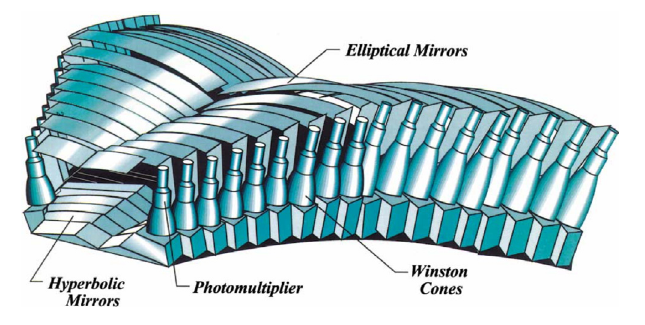
\includegraphics[width=\linewidth]{213ltcc.png}}
        \caption[LTCC Mirror System]{Layout and components of the optical mirror system within each LTCC box from the design model.}
        \label{fig::ltcc}
    \end{wrapfigure}

    The LTCC was a detector used in CLAS, which as part of the 12 GeV upgrade was refurbished to provide higher efficiency for charged pion and kaon detection.
    This was done by increasing the volume of the radiator gas, refurbishing the elliptical and hyperbolic mirrors with new coatings, and improving the sensitivity of the PMTs to Cherenkov light.
    The sensitivity improvement was achieved by coating their entrance windows with wavelength shifting material that absorbs ultraviolet (UV) light at wavelength below $300 ~\text{nm}$ and re-emits two back-to-back photons at larger wavelength \cite{ungaro2020}.
    A drawing from the design model of the LTCC can be seen in Figure \ref{fig::ltcc}.
